\documentclass[titlepage, a4paper, 11pt, dvipdfmx]{jsarticle}
\usepackage{customstyle}

\title{\Huge【レポート\#2】スプライン補間}%タイトル
\date{\today}%日付
\author{\Large BV20036 \quad 大野 弘貴}%名前

\begin{document}
\maketitle
\pagenumbering{roman}
% \tableofcontents%目次が消したい場合はコメントアウト
\newpage
\pagenumbering{arabic}

%%%%%%%%%%%%%%%%%%%%%%%%%%%%%%%%%%%%%%%%%%%%%%%%%%%%%%%%%%%%%%%%%%%%%%%%%%%%%
%%%%%%%%%%%%%%%%%%%%%%%%%%%%%%%%%%%%%%%%%%%%%%%%%%%%%%%%%%%%%%%%%%%%%%%%%%%%%
%%%%%%%%%%%%%%%%%%%%%%%%%%%%%%%%%%%%%%%%%%%%%%%%%%%%%%%%%%%%%%%%%%%%%%%%%%%%%
%以下サンプル%ここから書き始めてください

%セクション(目次に表示されるのは初期設定では)
\section{レポート内容}
\begin{itembox}[l]{レポート内容【スプライン補間】}
    \begin{itemize}
      \item[(1)]真の関数および区間を適当に設定し、そこから標本点を与え、スプライン補間を求める
      \item[(2)]標本点の数を適当に変え、スプライン補間で得られるグラフの概形の変化を調べる
      \item[(3)](1)において、真の関数値とスプライン補間によって得られた関数値のゴザをグラフに表示  
        \item 上記の(1),(2),(3)を3種類以上の真の関数に対してそれぞれ行い,十分な考察を記入し,レポートにまとめること

        \begin{itemize}
            \item 3種類のうち1つは【レポート\#1】のラグランジュ補間で使用した以下の真の関数を用いること.(区間は[-5, 5])
        $$ f(x)=\frac{1}{1+2x^2} $$
        \end{itemize} 
        \item 真の関数としては,多項式,三角関数,指数関数,対数関数,及びそれらの組み合わせ等,異なる種類(形)を選ぶこと
  \end{itemize}
\end{itembox}
\section{スプライン補間とは}
ラグランジュの補間は次数が高くなると振動してしまう.そこで,全区間を小区間に分割し,小区間ごとにラグランジュ補間を行うことで振動がなくなることを元に考えられたのがスプライン補間である.


\begin{itembox}[l]{スプライン補間}
    \begin{itemize}
        \item スプライン補間
      $$ S(x) \coloneqq S_k(x) = a_k(x-x_k)^3 + b_k(x-x_k)^2 + c_k(x-x_k) + d_k,$$
      $$ x_k \le x \le x_{k+1}, k=0, 1, \cdots ,n-1 $$
      $$ S_{k}''(x_k) = u_k, k=0, 1, \cdots ,n $$
        \item 係数
      $$ a_k = \frac{u_{k+1}-u_k}{6(x_{k+1}-x_k)}, b_k = \frac{u_k}{2}, d_k = f_k $$
      $$ c_k = \frac{f_{k+1}-f_k}{x_{k+1}-x_k}-\frac{1}{6}(u_{k+1}+2u_k)(x_{k+1}-x_k) $$
        
  \end{itemize}
\end{itembox}

\newpage


\section{実装したコード}

%プログラム挿入
\lstinputlisting[caption=splinesample.m, label=Label_Program]{../../spline/spline_sample.m}%[キャプションやらラベルやら]{ファイルの相対パス}


%画像挿入
\begin{figure}[H]
  \begin{center}%中央寄せ用
    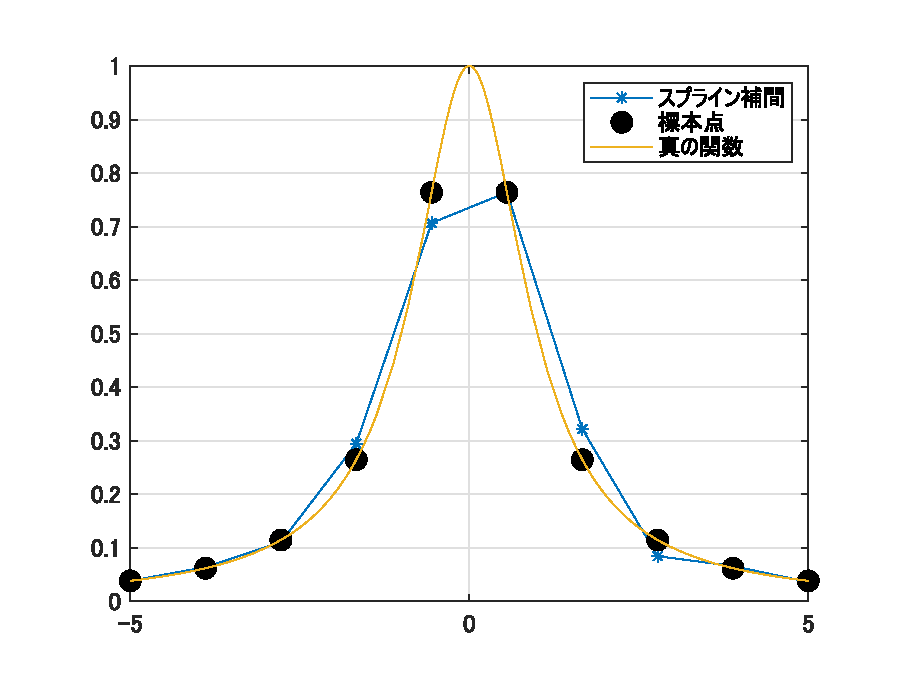
\includegraphics[width=13.5cm]{./graphics/s-1010.eps}%[大きさ指定]{ファイルの相対パス}
  \caption{標本点10 分割10}
  \label{Label}%ラベル
  \end{center}
\end{figure}

\begin{figure}[H]
  \begin{center}%中央寄せ用
    \includegraphics[width=13.5cm]{../../spline/910.eps}%[大きさ指定]{ファイルの相対パス}
  \caption{キャプション}
  \label{Label}%ラベル
  \end{center}
\end{figure}



\begin{figure}[H]
  \begin{center}%中央寄せ用
    \includegraphics[width=13.5cm]{../../spline/9909.eps}%[大きさ指定]{ファイルの相対パス}
  \caption{キャプション}
  \label{Label}%ラベル
  \end{center}
\end{figure}


\begin{figure}[H]
  \begin{center}%中央寄せ用
    \includegraphics[width=13.5cm]{../../spline/9910.eps}%[大きさ指定]{ファイルの相対パス}
  \caption{キャプション}
  \label{Label}%ラベル
  \end{center}
\end{figure}

\begin{figure}[H]
  \begin{center}%中央寄せ用
    \includegraphics[width=13.5cm]{../../spline/99909.eps}%[大きさ指定]{ファイルの相対パス}
  \caption{キャプション}
  \label{Label}%ラベル
  \end{center}
\end{figure}


\begin{figure}[H]
  \begin{center}%中央寄せ用
    \includegraphics[width=13.5cm]{../../spline/99910.eps}%[大きさ指定]{ファイルの相対パス}
  \caption{キャプション}
  \label{Label}%ラベル
  \end{center}
\end{figure}
分割数が同じでも標本が奇数のほうが正確なことである。また、分割数が図1のように分割数が少ない時はどちらも誤差も対して変わらなく大きくハズレている。また、分割数が多いほうが滑らかな1つの関数に見える。しかし標本点が奇数のときは、滑らかなことには変わりは無いが頂点の標本を通らずに少し潰れたグラフになっている。

\begin{figure}[H]
  \begin{center}%中央寄せ用
    \includegraphics[width=13.5cm]{../../spline/cs-9-9.eps}%[大きさ指定]{ファイルの相対パス}
  \caption{キャプション}
  \label{Label}%ラベル
  \end{center}
\end{figure}
大きくハズレている

\begin{figure}[H]
  \begin{center}%中央寄せ用
    \includegraphics[width=13.5cm]{../../spline/cs-9-10.eps}%[大きさ指定]{ファイルの相対パス}
  \caption{キャプション}
  \label{Label}%ラベル
  \end{center}
\end{figure}
大きくハズレている
\begin{figure}[H]
  \begin{center}%中央寄せ用
    \includegraphics[width=13.5cm]{../../spline/cs-99-9.eps}%[大きさ指定]{ファイルの相対パス}
  \caption{キャプション}
  \label{Label}%ラベル
  \end{center}
\end{figure}


頂点を通らず、ところどころカクカクになっている。

\begin{figure}[H]
  \begin{center}%中央寄せ用
    \includegraphics[width=13.5cm]{../../spline/cs-99-10.eps}%[大きさ指定]{ファイルの相対パス}
  \caption{キャプション}
  \label{Label}%ラベル
  \end{center}
\end{figure}

左右の頂点は通っていないが概ね近似できている

\begin{figure}[H]
  \begin{center}%中央寄せ用
    \includegraphics[width=13.5cm]{../../spline/cs-999-10.eps}%[大きさ指定]{ファイルの相対パス}
  \caption{キャプション}
  \label{Label}%ラベル
  \end{center}
\end{figure}

左右の頂点は通っていないが概ね近似できている。

\begin{figure}[H]
  \begin{center}%中央寄せ用
    \includegraphics[width=13.5cm]{../../spline/cs-999-9.eps}%[大きさ指定]{ファイルの相対パス}
  \caption{キャプション}
  \label{Label}%ラベル
  \end{center}
\end{figure}
頂点を通らず値が突然飛んでいる。

\begin{figure}[H]
  \begin{center}%中央寄せ用
    \includegraphics[width=13.5cm]{../../spline/e-9-9.eps}%[大きさ指定]{ファイルの相対パス}
  \caption{キャプション}
  \label{Label}%ラベル
  \end{center}
\end{figure}





\begin{figure}[H]
  \begin{center}%中央寄せ用
    \includegraphics[width=13.5cm]{../../spline/e-9-10.eps}%[大きさ指定]{ファイルの相対パス}
  \caption{キャプション}
  \label{Label}%ラベル
  \end{center}
\end{figure}


\begin{figure}[H]
  \begin{center}%中央寄せ用
    \includegraphics[width=13.5cm]{../../spline/e-99-9.eps}%[大きさ指定]{ファイルの相対パス}
  \caption{キャプション}
  \label{Label}%ラベル
  \end{center}
\end{figure}


\begin{figure}[H]
  \begin{center}%中央寄せ用
    \includegraphics[width=13.5cm]{../../spline/e-99-10.eps}%[大きさ指定]{ファイルの相対パス}
  \caption{キャプション}
  \label{Label}%ラベル
  \end{center}
\end{figure}


\begin{figure}[H]
  \begin{center}%中央寄せ用
    \includegraphics[width=13.5cm]{../../spline/e-999-9.eps}%[大きさ指定]{ファイルの相対パス}
  \caption{キャプション}
  \label{Label}%ラベル
  \end{center}
\end{figure}


\begin{figure}[H]
  \begin{center}%中央寄せ用
    \includegraphics[width=13.5cm]{../../spline/e-999-10.eps}%[大きさ指定]{ファイルの相対パス}
  \caption{キャプション}
  \label{Label}%ラベル
  \end{center}
\end{figure}

誤差
\begin{figure}[H]
  \begin{center}%中央寄せ用
    \includegraphics[width=13.5cm]{../../spline/abs-99.eps}%[大きさ指定]{ファイルの相対パス}
  \caption{キャプション}
  \label{Label}%ラベル
  \end{center}
\end{figure}


\begin{figure}[H]
  \begin{center}%中央寄せ用
    \includegraphics[width=13.5cm]{../../spline/e-abs-99.eps}%[大きさ指定]{ファイルの相対パス}
  \caption{キャプション}
  \label{Label}%ラベル
  \end{center}
\end{figure}


\begin{figure}[H]
  \begin{center}%中央寄せ用
    \includegraphics[width=13.5cm]{../../spline/cs-abs-99.eps}%[大きさ指定]{ファイルの相対パス}
  \caption{キャプション}
  \label{Label}%ラベル
  \end{center}
\end{figure}

  %ラベルは\ref{Label}のように書くと数字だけ表示される(2回コンパイルが必要). {括弧}の中身は任意(英語推奨).

\section{考察}
最初の関数
まず、標本点が奇数の場合、標本点は真の関数の極大値を通る。そのため、標本点が奇数のときは近似式は極大値を通りうまく近似できている。しかし分割数が極端に少ない場合は各頂点を通るだけの分割数がないためうまく近似できていないことが分かる。
2個目の関数
まず、標本点が奇数の場合、標本点は端の極大値を除き真の関数の極大値を通る。これも最初の関数と同様のことが言える。
3個目
無理数であるeを用いた指数関数なら突飛なが起きるかもしれないと考えたが、eはたかが定数であるからグラフ自体も簡単であるから何も起きずに近似された。この式には頂点が無いので、奇数偶数のときに関わらず同じように分割数を増やせばより良い近似式が得られた。有効桁を指定すれば無理数も有理数と同じなので変なことが起きなかったのかもしれない。

誤差に関しては自然スプランにしたせいか、両端が大きくハズレる形になっている。



\end{document}
